% 1
%\documentclass[12pt]{article}
%\usepackage[letterpaper, margin=1in]{geometry}
%\usepackage{fancyhdr}
%\usepackage{titlesec}
%\usepackage{lmodern}
%\usepackage{xcolor}
%\usepackage{hyperref}
%\usepackage{enumitem}
%\usepackage{amsmath, amssymb, amsthm}
%\usepackage{kotex} % for Korean support
%
%% Define a primary color for links and headings
%\definecolor{primary}{RGB}{0,102,204}
%\hypersetup{
%	colorlinks=true,
%	linkcolor=primary,
%	urlcolor=primary,
%}
%
%% Setup fancy header and footer
%\pagestyle{fancy}
%\fancyhf{}
%\lhead{\textbf{Graduate-Level Mathematics Syllabus / 대학원 수준 수학 강의계획서}}
%\rhead{\thepage}
%\renewcommand{\headrulewidth}{2pt}
%\renewcommand{\footrulewidth}{1pt}
%
%% Title formatting for sections and subsections
%\titleformat{\section}{\normalfont\Large\bfseries}{\thesection}{1em}{}
%\titleformat{\subsection}{\normalfont\large\bfseries}{\thesubsection}{1em}{}
%
%\begin{document}
%	
%	\begin{center}
%		{\Huge \textbf{Graduate-Level Mathematics Syllabus \\ 대학원 수준 수학 강의계획서}}\\[0.5cm]
%		{\Large Department of Mathematics / 수학과}\\[0.2cm]
%		{\large Academic Year 2025--2026 / 2025--2026 학년도}\\[1cm]
%	\end{center}
%	
%	\hrulefill
%	
%	\section*{Course Overview / 강의 개요}
%	This comprehensive course is designed to bridge the gap between undergraduate and graduate-level mathematics. The curriculum includes an in-depth exploration of fundamental areas such as Set Theory, Real Analysis, Topology, Linear Algebra, and Abstract Algebra.
%	\\[1em]
%	이 포괄적인 강의는 학부 수준의 수학과 대학원 수준의 수학 사이의 격차를 줄이기 위해 설계되었습니다. 강의 내용에는 집합론, 실해석, 위상수학, 선형대수학, 추상대수학과 같은 기본 영역의 심도 있는 탐구가 포함됩니다.
%	
%	\section*{Course Objectives / 강의 목표}
%	\begin{itemize}[leftmargin=*, label={--}]
%		\item Develop a deep understanding of foundational mathematical concepts.
%		\item Transition smoothly from undergraduate to advanced mathematical thinking.
%		\item Enhance skills in constructing rigorous proofs and solving complex problems.
%		\item Explore the interconnections among various branches of mathematics.
%	\end{itemize}
%	\begin{itemize}[leftmargin=*, label={--}]
%		\item 기본 수학 개념에 대한 깊은 이해를 발전시킵니다.
%		\item 학부 수준에서 고급 수학적 사고로 원활하게 전환합니다.
%		\item 엄격한 증명 구성 및 복잡한 문제 해결 능력을 향상시킵니다.
%		\item 다양한 수학 분야 간의 상호 연결성을 탐구합니다.
%	\end{itemize}
%	
%	\section*{Textbooks and Materials / 교재 및 자료}
%	\begin{enumerate}[label=\arabic*.]
%		\item \textbf{Set Theory / 집합론:} \emph{Naive Set Theory} by Paul R. Halmos.
%		\item \textbf{Real Analysis / 실해석:} \emph{Principles of Mathematical Analysis} by Walter Rudin.
%		\item \textbf{Topology / 위상수학:} \emph{Topology} by James R. Munkres.
%		\item \textbf{Linear Algebra / 선형대수학:} \emph{Linear Algebra Done Right} by Sheldon Axler.
%		\item \textbf{Abstract Algebra / 추상대수학:} \emph{Abstract Algebra} by David S. Dummit and Richard M. Foote.
%	\end{enumerate}
%	
%	\section*{Course Outline and Schedule / 강의 일정 및 내용}
%	\begin{enumerate}[label=\textbf{Week \arabic*:}, leftmargin=*, itemsep=1em]
%		\item \textbf{Introduction and Overview / 강의 소개 및 개요} \\
%		Topics: Course introduction, academic expectations, and review of foundational topics. \\
%		주제: 강의 소개, 학업 기대사항, 기본 주제 복습.
%		
%		\item \textbf{Set Theory / 집합론} \\
%		Topics: Basic set operations, functions, relations, cardinality, and an introduction to axiomatic set theory. \\
%		주제: 집합의 기본 연산, 함수, 관계, 기수, 공리적 집합론 소개.
%		
%		\item \textbf{Real Analysis I / 실해석 I} \\
%		Topics: Structure of the real number system, sequences, series, limits, and continuity. \\
%		주제: 실수 체계의 구조, 수열, 급수, 극한, 연속성.
%		
%		\item \textbf{Real Analysis II / 실해석 II} \\
%		Topics: Differentiation, integration, sequences of functions, and uniform convergence. \\
%		주제: 미분, 적분, 함수열, 균등 수렴.
%		
%		\item \textbf{Topology I / 위상수학 I} \\
%		Topics: Metric spaces, open and closed sets, bases for a topology, continuity, and compactness. \\
%		주제: 거리 공간, 열린 집합 및 닫힌 집합, 위상의 기저, 연속성, 콤팩트성.
%		
%		\item \textbf{Topology II / 위상수학 II} \\
%		Topics: Connectedness, path-connectedness, the fundamental group, and introductory algebraic topology. \\
%		주제: 연결성, 경로 연결성, 기본군, 기초 대수적 위상수학.
%		
%		\item \textbf{Linear Algebra I / 선형대수학 I} \\
%		Topics: Vector spaces, linear transformations, matrices, and systems of linear equations. \\
%		주제: 벡터 공간, 선형 변환, 행렬, 연립 선형 방정식.
%		
%		\item \textbf{Linear Algebra II / 선형대수학 II} \\
%		Topics: Eigenvalues, eigenvectors, diagonalization, and inner product spaces. \\
%		주제: 고유값, 고유벡터, 대각화, 내적 공간.
%		
%		\item \textbf{Abstract Algebra I / 추상대수학 I} \\
%		Topics: Groups, subgroups, cyclic groups, and group homomorphisms. \\
%		주제: 군, 부분군, 순환군, 군 준동형.
%		
%		\item \textbf{Abstract Algebra II / 추상대수학 II} \\
%		Topics: Rings, ideals, ring homomorphisms, and an introduction to fields and modules. \\
%		주제: 환, 아이디얼, 환 준동형, 필드와 가군 소개.
%		
%		\item \textbf{Integration of Concepts / 개념의 통합} \\
%		Topics: Interdisciplinary projects and advanced topics integrating various mathematical disciplines. \\
%		주제: 다양한 수학 분야를 통합하는 학제 간 프로젝트 및 심화 주제.
%		
%		\item \textbf{Final Review and Assessment / 최종 복습 및 평가} \\
%		Topics: Comprehensive review, problem-solving sessions, and final examinations. \\
%		주제: 종합 복습, 문제 해결 세션, 최종 평가.
%	\end{enumerate}
%	
%	\section*{Grading Policy / 평가 기준}
%	\begin{itemize}[leftmargin=*, label={--}]
%		\item \textbf{Assignments / 과제:} 30\% (Regular homework and project work / 정기 과제 및 프로젝트)
%		\item \textbf{Midterm Examinations / 중간고사:} 30\%
%		\item \textbf{Final Examination / 기말고사:} 40\%
%	\end{itemize}
%	
%	\section*{Additional Information / 추가 정보}
%	\begin{itemize}[leftmargin=*, label={--}]
%		\item Regular office hours will be held weekly. \quad (정기 상담 시간이 주간에 제공됩니다.)
%		\item Collaborative work is encouraged; however, all submitted work must be the student’s own. \quad (협업이 권장되지만, 제출된 모든 작업은 학생 본인의 것이어야 합니다.)
%		\item Attendance, active participation, and timely submission of assignments are expected. \quad (출석, 적극적인 참여 및 과제의 기한 내 제출이 요구됩니다.)
%	\end{itemize}
%	
%	\hrulefill
%	
%	\begin{center}
%		\textbf{Department of Mathematics / 수학과} \\
%		\textit{University Name / 대학교 이름} \\
%		\textit{Contact: email@university.edu}
%	\end{center}
%	
%\end{document}













% 2
%\documentclass[12pt]{article}
%\usepackage[letterpaper, margin=1in]{geometry}
%\usepackage{fancyhdr}
%\usepackage{titlesec}
%\usepackage{lmodern}
%\usepackage{hyperref}
%\usepackage{enumitem}
%\usepackage{amsmath, amssymb, amsthm}
%\usepackage{kotex} % for Korean text support
%
%% Setup header and footer
%\pagestyle{fancy}
%\fancyhf{}
%\lhead{\textbf{Graduate-Level Mathematics Syllabus / 대학원 수준 수학 강의계획서}}
%\rhead{\thepage}
%\renewcommand{\headrulewidth}{1pt}
%\renewcommand{\footrulewidth}{0pt}
%
%% Section formatting
%\titleformat{\section}{\normalfont\Large\bfseries}{\thesection}{1em}{}
%\titleformat{\subsection}{\normalfont\large\bfseries}{\thesubsection}{1em}{}
%
%\begin{document}
%	
%	\begin{center}
%		{\Huge \textbf{Graduate-Level Mathematics Syllabus \\ 대학원 수준 수학 강의계획서}}\\[0.5cm]
%		{\Large Department of Mathematics / 수학과}\\[0.2cm]
%		{\large Academic Year 2025--2026 / 2025--2026 학년도}\\[1cm]
%	\end{center}
%	
%	\hrule
%	
%	\section*{Course Overview / 강의 개요}
%	This course offers a comprehensive exploration of graduate-level mathematics, bridging the gap from undergraduate studies. The topics include set theory, advanced calculus, topology, and algebraic structures.
%	\\[1em]
%	이 강의는 학부 수준의 수학에서 대학원 수준의 수학으로의 다리를 제공하며, 집합론, 고급 해석학, 위상수학, 대수 구조 등을 포괄적으로 다룹니다.
%	
%	\section*{Course Objectives / 강의 목표}
%	\begin{itemize}[leftmargin=*, label={--}]
%		\item Develop advanced mathematical reasoning and rigorous proof techniques.
%		\item Deepen understanding of fundamental mathematical theories.
%		\item Integrate concepts across various mathematical disciplines.
%	\end{itemize}
%	\begin{itemize}[leftmargin=*, label={--}]
%		\item 고급 수학적 사고와 엄격한 증명 기법을 개발합니다.
%		\item 기본 수학 이론에 대한 이해를 심화합니다.
%		\item 다양한 수학 분야의 개념을 통합합니다.
%	\end{itemize}
%	
%	\section*{Lecture Notes Overview / 강의 노트 개요}
%	Below is an outline of the lecture note files and the topics covered in each.
%	\\[1em]
%	다음은 강의 노트 파일별로 다루는 주제의 개요입니다.
%	
%	\subsection*{grad-math-1.tex/pdf: Set Theory I / 집합론 I}
%	\begin{itemize}[leftmargin=*, label={--}]
%		\item Set, Power Set, Cartesian Product
%		\item Union, Intersection, Complement
%		\item Function, Image, Pre-image
%		\item Injection, Surjection, Bijection
%		\item Axiom of Choice
%	\end{itemize}
%	
%	\subsection*{grad-math-2.tex/pdf: Set Theory II / 집합론 II}
%	\begin{itemize}[leftmargin=*, label={--}]
%		\item Relation, Equivalence Relation
%		\item Equivalence Class, Partition
%	\end{itemize}
%	
%	\subsection*{grad-math-3.tex/pdf: Advanced Calculus I / 고급 해석학 I}
%	\begin{itemize}[leftmargin=*, label={--}]
%		\item Boundedness, Supremum and Infimum
%		\item Least Upper Bound Property (Completeness Axiom)
%		\item Well-Ordering Principle and Mathematical Induction
%		\item Archimedean Property
%	\end{itemize}
%	
%	\subsection*{grad-math-4.tex/pdf: Advanced Calculus II / 고급 해석학 II}
%	\begin{itemize}[leftmargin=*, label={--}]
%		\item Convergence of Sequences
%		\item Inequality Rule for Absolute Values
%		\item Limit Theorem (Algebraic Property of Limit of Sequence)
%	\end{itemize}
%	
%	\subsection*{grad-math-5.tex/pdf: Topology I / 위상수학 I}
%	\begin{itemize}[leftmargin=*, label={--}]
%		\item Topology and Topological Space
%		\item Open Set
%		\item Continuous Mapping
%		\item Distance Function and Metric Space
%		\item Convergence of Sequences; Continuity of Functions
%	\end{itemize}
%	
%	\subsection*{grad-math-6.tex/pdf: Advanced Calculus III / 고급 해석학 III}
%	\begin{itemize}[leftmargin=*, label={--}]
%		\item Limit of a Function
%		\item Continuity of a Function
%		\item Monotone Convergence Theorem (MCT)
%		\item Nested Interval Property (NIP)
%		\item Bolzano-Weierstrass Theorem
%		\item Limit Superior and Limit Inferior
%	\end{itemize}
%	
%	\subsection*{grad-math-7.tex/pdf: Algebraic Structures / 대수 구조}
%	\begin{itemize}[leftmargin=*, label={--}]
%		\item Group
%		\item Ring
%		\item Field
%		\item Module
%		\item Vector Space
%		\item Algebra
%	\end{itemize}
%	
%	\section*{Grading Policy / 평가 기준}
%	\begin{itemize}[leftmargin=*, label={--}]
%		\item Assignments: 30\%
%		\item Midterm Examinations: 30\%
%		\item Final Examination: 40\%
%	\end{itemize}
%	\begin{itemize}[leftmargin=*, label={--}]
%		\item 과제: 30\%
%		\item 중간고사: 30\%
%		\item 기말고사: 40\%
%	\end{itemize}
%	
%	\section*{Additional Information / 추가 정보}
%	\begin{itemize}[leftmargin=*, label={--}]
%		\item Regular office hours will be provided.
%		\item Collaboration is encouraged; however, all submitted work must be individual.
%	\end{itemize}
%	\begin{itemize}[leftmargin=*, label={--}]
%		\item 정기 상담 시간이 제공됩니다.
%		\item 협업은 권장되나, 제출된 작업은 개인별로 이루어져야 합니다.
%	\end{itemize}
%	
%	\hrule
%	
%	\begin{center}
%		\textbf{Department of Mathematics / 수학과} \\
%		\textit{University Name / 대학교 이름} \\
%		\textit{Contact: email@university.edu}
%	\end{center}
%	
%\end{document}









% 3
%\documentclass[12pt]{article}
%\usepackage[letterpaper, margin=1in]{geometry}
%\usepackage{fancyhdr}
%\usepackage{titlesec}
%\usepackage{lmodern}
%\usepackage{hyperref}
%\usepackage{enumitem}
%\usepackage{amsmath, amssymb, amsthm}
%\usepackage{kotex} % for Korean text support
%
%% Setup header and footer
%\pagestyle{fancy}
%\fancyhf{}
%\lhead{\textbf{Foundations and Frontiers of Modern Mathematics / 현대 수학의 기초와 최전선}}
%\rhead{\thepage}
%\renewcommand{\headrulewidth}{1pt}
%\renewcommand{\footrulewidth}{0pt}
%
%% Section formatting
%\titleformat{\section}{\normalfont\Large\bfseries}{\thesection}{1em}{}
%\titleformat{\subsection}{\normalfont\large\bfseries}{\thesubsection}{1em}{}
%
%\begin{document}
%	
%	\begin{center}
%		{\Huge \textbf{Foundations and Frontiers of Modern Mathematics \\ 현대 수학의 기초와 최전선}}\\[0.5cm]
%		{\Large Department of Mathematics / 수학과}\\[0.2cm]
%		{\large Academic Year 2025--2026 / 2025--2026 학년도}\\[1cm]
%	\end{center}
%	
%	\hrule
%	
%	\section*{Course Overview / 강의 개요}
%	This course offers a comprehensive journey through modern mathematical theories, seamlessly bridging foundational concepts with advanced topics. Emphasizing rigorous reasoning, the curriculum delves into set theory, advanced calculus, topology, and algebraic structures, setting the stage for both theoretical exploration and practical applications.
%	\\[1em]
%	이 강의는 현대 수학 이론을 포괄적으로 탐구하며, 기초 개념과 고급 주제를 원활하게 연결합니다. 엄격한 논리 전개를 강조하며, 강의 내용은 집합론, 고급 해석학, 위상수학, 대수 구조를 다루어 이론적 탐구와 실제 응용의 기초를 마련합니다.
%	
%	\section*{Course Objectives / 강의 목표}
%	\begin{itemize}[leftmargin=*, label={--}]
%		\item Develop advanced mathematical reasoning and rigorous proof techniques.
%		\item Deepen understanding of fundamental mathematical theories.
%		\item Integrate concepts across various mathematical disciplines.
%	\end{itemize}
%	\begin{itemize}[leftmargin=*, label={--}]
%		\item 고급 수학적 사고와 엄격한 증명 기법을 개발합니다.
%		\item 기본 수학 이론에 대한 이해를 심화합니다.
%		\item 다양한 수학 분야의 개념을 통합합니다.
%	\end{itemize}
%	
%	\section*{Lecture Notes Overview / 강의 노트 개요}
%	Below is an outline of the lecture note files and the topics covered in each.
%	\\[1em]
%	다음은 강의 노트 파일별로 다루는 주제의 개요입니다.
%	
%	\subsection*{grad-math-1.tex/pdf: Set Theory I / 집합론 I}
%	\begin{itemize}[leftmargin=*, label={--}]
%		\item Set, Power Set, Cartesian Product
%		\item Union, Intersection, Complement
%		\item Function, Image, Pre-image
%		\item Injection, Surjection, Bijection
%		\item Axiom of Choice
%	\end{itemize}
%	
%	\subsection*{grad-math-2.tex/pdf: Set Theory II / 집합론 II}
%	\begin{itemize}[leftmargin=*, label={--}]
%		\item Relation, Equivalence Relation
%		\item Equivalence Class, Partition
%	\end{itemize}
%	
%	\subsection*{grad-math-3.tex/pdf: Advanced Calculus I / 고급 해석학 I}
%	\begin{itemize}[leftmargin=*, label={--}]
%		\item Boundedness, Supremum and Infimum
%		\item Least Upper Bound Property (Completeness Axiom)
%		\item Well-Ordering Principle and Mathematical Induction
%		\item Archimedean Property
%	\end{itemize}
%	
%	\subsection*{grad-math-4.tex/pdf: Advanced Calculus II / 고급 해석학 II}
%	\begin{itemize}[leftmargin=*, label={--}]
%		\item Convergence of Sequences
%		\item Inequality Rule for Absolute Values
%		\item Limit Theorem (Algebraic Property of Limit of Sequence)
%	\end{itemize}
%	
%	\subsection*{grad-math-5.tex/pdf: Topology I / 위상수학 I}
%	\begin{itemize}[leftmargin=*, label={--}]
%		\item Topology and Topological Space
%		\item Open Set
%		\item Continuous Mapping
%		\item Distance Function and Metric Space
%		\item Convergence of Sequences; Continuity of Functions
%	\end{itemize}
%	
%	\subsection*{grad-math-6.tex/pdf: Advanced Calculus III / 고급 해석학 III}
%	\begin{itemize}[leftmargin=*, label={--}]
%		\item Limit of a Function
%		\item Continuity of a Function
%		\item Monotone Convergence Theorem (MCT)
%		\item Nested Interval Property (NIP)
%		\item Bolzano-Weierstrass Theorem
%		\item Limit Superior and Limit Inferior
%	\end{itemize}
%	
%	\subsection*{grad-math-7.tex/pdf: Algebraic Structures / 대수 구조}
%	\begin{itemize}[leftmargin=*, label={--}]
%		\item Group
%		\item Ring
%		\item Field
%		\item Module
%		\item Vector Space
%		\item Algebra
%	\end{itemize}
%	
%	\section*{Grading Policy / 평가 기준}
%	\begin{itemize}[leftmargin=*, label={--}]
%		\item Assignments: 30\%
%		\item Midterm Examinations: 30\%
%		\item Final Examination: 40\%
%	\end{itemize}
%	\begin{itemize}[leftmargin=*, label={--}]
%		\item 과제: 30\%
%		\item 중간고사: 30\%
%		\item 기말고사: 40\%
%	\end{itemize}
%	
%	\section*{Additional Information / 추가 정보}
%	\begin{itemize}[leftmargin=*, label={--}]
%		\item Regular office hours will be provided.
%		\item Collaboration is encouraged; however, all submitted work must be individual.
%	\end{itemize}
%	\begin{itemize}[leftmargin=*, label={--}]
%		\item 정기 상담 시간이 제공됩니다.
%		\item 협업은 권장되나, 제출된 작업은 개인별로 이루어져야 합니다.
%	\end{itemize}
%	
%	\hrule
%	
%	\begin{center}
%		\textbf{Department of Mathematics / 수학과} \\
%		\textit{University Name / 대학교 이름} \\
%		\textit{Contact: email@university.edu}
%	\end{center}
%	
%\end{document}



% 4
%\documentclass[12pt]{article}
%\usepackage[letterpaper, margin=1in]{geometry}
%\usepackage{fancyhdr}
%\usepackage{titlesec}
%\usepackage{lmodern}
%\usepackage{hyperref}
%\usepackage{enumitem}
%\usepackage{amsmath, amssymb, amsthm}
%\usepackage{kotex} % Korean language support
%
%% Setup header and footer
%\pagestyle{fancy}
%\fancyhf{}
%\lhead{\textbf{Foundations and Frontiers of Modern Mathematics / 현대 수학의 기초와 최전선}}
%\rhead{\thepage}
%\renewcommand{\headrulewidth}{1pt}
%\renewcommand{\footrulewidth}{0pt}
%
%% Section formatting
%\titleformat{\section}{\normalfont\Large\bfseries}{\thesection}{1em}{}
%\titleformat{\subsection}{\normalfont\large\bfseries}{\thesubsection}{1em}{}
%
%\begin{document}
%	
%	\begin{center}
%		{\Huge \textbf{Foundations and Frontiers of Modern Mathematics \\ 현대 수학의 기초와 최전선}}\\[0.5cm]
%		{\Large Department of Mathematics / 수학과}\\[0.2cm]
%		{\large Academic Year 2025--2026 / 2025--2026 학년도}\\[1cm]
%	\end{center}
%	
%	\hrule
%	
%	\section*{Course Overview / 강의 개요}
%	The \textbf{Foundations and Frontiers of Modern Mathematics} course is an intensive, research-driven program designed for exceptionally motivated individuals seeking to deepen their expertise in modern mathematical theories. This program seamlessly integrates rigorous foundational concepts with contemporary topics, preparing participants for both advanced academic research and high-level professional practice. Core areas include set theory, advanced calculus, topology, and algebraic structures, all taught through an inquiry-based, collaborative approach.
%	\\[1em]
%	\textbf{현대 수학의 기초와 최전선} 강의는 현대 수학 이론에 대한 전문 지식을 심화하려는 우수한 인재들을 위해 설계된 집중적이며 연구 지향적인 프로그램입니다. 이 프로그램은 엄격한 기초 개념과 최신 주제를 원활하게 통합하여, 참가자들이 학문 연구와 고급 전문 실무 양쪽 모두에 대비할 수 있도록 합니다. 주요 분야로는 집합론, 고급 해석학, 위상수학, 대수 구조 등이 있으며, 탐구 기반의 협업 학습을 통해 진행됩니다.
%	
%	\section*{Course Objectives / 강의 목표}
%	\begin{itemize}[leftmargin=*, label={--}]
%		\item Cultivate advanced mathematical reasoning and mastery of rigorous proof techniques.
%		\item Deepen understanding of fundamental theories across key areas of modern mathematics.
%		\item Foster interdisciplinary integration and innovative problem-solving skills.
%		\item Prepare participants for future academic research or high-level professional endeavors.
%	\end{itemize}
%	\begin{itemize}[leftmargin=*, label={--}]
%		\item 고급 수학적 사고와 엄격한 증명 기법의 숙달.
%		\item 현대 수학의 주요 분야에 걸친 기본 이론에 대한 심도 있는 이해 증진.
%		\item 학제 간 통합과 혁신적 문제 해결 능력 함양.
%		\item 참가자들이 향후 학문 연구 또는 고급 전문 분야에서 성공할 수 있도록 준비.
%	\end{itemize}
%	
%	\section*{Target Audience and Application / 대상 및 지원 안내}
%	This course is open to graduate students, postgraduates, and professionals with a solid foundation in undergraduate mathematics who are eager to engage in advanced study and research. Prospective candidates should demonstrate strong analytical skills, a passion for mathematical inquiry, and the capacity for independent, creative thought.
%	\\[1em]
%	이 강의는 학부 수학의 기초가 탄탄한 대학원생, 박사후 연구원 및 전문가를 대상으로 하며, 고급 학문 연구 및 심화 학습에 열정을 가진 분들을 환영합니다. 지원자는 뛰어난 분석력, 수학적 탐구에 대한 열정, 그리고 독립적이고 창의적인 사고 능력을 갖추어야 합니다.
%	
%	\section*{Lecture Notes Overview / 강의 노트 개요}
%	The curriculum is organized into a series of comprehensive lecture notes, each focusing on a specific facet of modern mathematics. The following outlines the topics covered in each file:
%	\\[1em]
%	커리큘럼은 현대 수학의 특정 측면에 초점을 맞춘 일련의 강의 노트로 구성되어 있습니다. 각 파일에서 다루는 주제는 다음과 같습니다.
%	
%	\subsection*{grad-math-1.tex/pdf: Set Theory I / 집합론 I}
%	\begin{itemize}[leftmargin=*, label={--}]
%		\item Set, Power Set, Cartesian Product
%		\item Union, Intersection, Complement
%		\item Function, Image, Pre-image
%		\item Injection, Surjection, Bijection
%		\item Axiom of Choice
%	\end{itemize}
%	
%	\subsection*{grad-math-2.tex/pdf: Set Theory II / 집합론 II}
%	\begin{itemize}[leftmargin=*, label={--}]
%		\item Relation, Equivalence Relation
%		\item Equivalence Class, Partition
%	\end{itemize}
%	
%	\subsection*{grad-math-3.tex/pdf: Advanced Calculus I / 고급 해석학 I}
%	\begin{itemize}[leftmargin=*, label={--}]
%		\item Boundedness, Supremum and Infimum
%		\item Least Upper Bound Property (Completeness Axiom)
%		\item Well-Ordering Principle and Mathematical Induction
%		\item Archimedean Property
%	\end{itemize}
%	
%	\subsection*{grad-math-4.tex/pdf: Advanced Calculus II / 고급 해석학 II}
%	\begin{itemize}[leftmargin=*, label={--}]
%		\item Convergence of Sequences
%		\item Inequality Rule for Absolute Values
%		\item Limit Theorem (Algebraic Property of Limit of Sequence)
%	\end{itemize}
%	
%	\subsection*{grad-math-5.tex/pdf: Topology I / 위상수학 I}
%	\begin{itemize}[leftmargin=*, label={--}]
%		\item Topology and Topological Space
%		\item Open Set
%		\item Continuous Mapping
%		\item Distance Function and Metric Space
%		\item Convergence of Sequences; Continuity of Functions
%	\end{itemize}
%	
%	\subsection*{grad-math-6.tex/pdf: Advanced Calculus III / 고급 해석학 III}
%	\begin{itemize}[leftmargin=*, label={--}]
%		\item Limit of a Function
%		\item Continuity of a Function
%		\item Monotone Convergence Theorem (MCT)
%		\item Nested Interval Property (NIP)
%		\item Bolzano-Weierstrass Theorem
%		\item Limit Superior and Limit Inferior
%	\end{itemize}
%	
%	\subsection*{grad-math-7.tex/pdf: Algebraic Structures / 대수 구조}
%	\begin{itemize}[leftmargin=*, label={--}]
%		\item Group
%		\item Ring
%		\item Field
%		\item Module
%		\item Vector Space
%		\item Algebra
%	\end{itemize}
%	
%	\section*{Program Structure and Assessment / 프로그램 구조 및 평가}
%	This program combines rigorous coursework with interactive seminars and independent research projects. Assessment will be based on:
%	\begin{itemize}[leftmargin=*, label={--}]
%		\item Comprehensive written assignments and research proposals.
%		\item In-depth midterm examinations.
%		\item A final comprehensive examination.
%	\end{itemize}
%	\begin{itemize}[leftmargin=*, label={--}]
%		\item 서면 과제 및 연구 제안서.
%		\item 심도 있는 중간고사.
%		\item 종합 기말고사.
%	\end{itemize}
%	
%	\section*{Application Process / 지원 절차}
%	Prospective candidates are invited to submit the following:
%	\begin{itemize}[leftmargin=*, label={--}]
%		\item A detailed curriculum vitae.
%		\item A statement of purpose outlining research interests and career goals.
%		\item Official academic transcripts.
%		\item Two letters of recommendation.
%	\end{itemize}
%%	\\[0.5em]
%	지원자는 다음 서류를 제출해 주시기 바랍니다:
%	\begin{itemize}[leftmargin=*, label={--}]
%		\item 상세한 이력서.
%		\item 연구 관심사 및 경력 목표를 기술한 자기소개서.
%		\item 공식 성적 증명서.
%		\item 추천서 2부.
%	\end{itemize}
%	
%	\section*{Additional Information / 추가 정보}
%	\begin{itemize}[leftmargin=*, label={--}]
%		\item Regular office hours and consultation sessions will be available.
%		\item Collaborative research initiatives are highly encouraged.
%		\item Prospective candidates are welcome to attend an introductory seminar session.
%	\end{itemize}
%	\begin{itemize}[leftmargin=*, label={--}]
%		\item 정기 상담 시간과 개별 상담이 제공됩니다.
%		\item 협업 연구가 적극 권장됩니다.
%		\item 지원자들은 소개 세미나에 참석할 수 있습니다.
%	\end{itemize}
%	
%	\hrule
%	
%	\begin{center}
%		\textbf{Department of Mathematics / 수학과} \\
%		\textit{University Name / 대학교 이름} \\
%		\textit{Contact: email@university.edu}
%	\end{center}
%	
%\end{document}


% 5
%\documentclass[12pt]{article}
%\usepackage[letterpaper, margin=1in]{geometry}
%\usepackage{fancyhdr}
%\usepackage{titlesec}
%\usepackage{lmodern}
%\usepackage{hyperref}
%\usepackage{enumitem}
%\usepackage{amsmath, amssymb, amsthm}
%\usepackage{kotex} % for Korean language support
%
%% Setup header and footer
%\pagestyle{fancy}
%\fancyhf{}
%\lhead{\textbf{Foundations and Frontiers of Modern Mathematics / 현대 수학의 기초와 최전선}}
%\rhead{\thepage}
%\renewcommand{\headrulewidth}{1pt}
%\renewcommand{\footrulewidth}{0pt}
%
%% Section formatting
%\titleformat{\section}{\normalfont\Large\bfseries}{\thesection}{1em}{}
%\titleformat{\subsection}{\normalfont\large\bfseries}{\thesubsection}{1em}{}
%
%\begin{document}
%	
%	\begin{center}
%		{\Huge \textbf{Foundations and Frontiers of Modern Mathematics \\ 현대 수학의 기초와 최전선}}\\[0.5cm]
%		{\Large Department of Mathematics / 수학과}\\[0.2cm]
%		{\large Academic Year 2025--2026 / 2025--2026 학년도}\\[1cm]
%	\end{center}
%	
%	\hrule
%	
%	\section*{Course Overview / 강의 개요}
%	Mathematics has a way of telling stories—stories of discovery, logical beauty, and endless curiosity. \textbf{Foundations and Frontiers of Modern Mathematics} is designed to make the often intimidating world of graduate-level math both accessible and enjoyable. This course welcomes participants regardless of academic grade—whether you are an undergraduate, a graduate student, or simply a math enthusiast—our aim is to create a vibrant community where we learn, share, and delight in the rich narratives of mathematics.  
%	\\[1em]
%	수학은 발견, 논리의 아름다움, 그리고 끝없는 호기심의 이야기를 들려줍니다. \textbf{현대 수학의 기초와 최전선} 강의는 대학원 수준의 수학을 쉽고 즐겁게 접근할 수 있도록 설계되었습니다. 이 강의는 학부생, 대학원생은 물론 수학을 사랑하는 모든 분들을 환영하며, 함께 모여 수학의 풍부한 이야기를 배우고 나누며 즐기는 공동체를 만드는 것이 목표입니다.
%	
%	\section*{Course Objectives / 강의 목표}
%	\begin{itemize}[leftmargin=*, label={--}]
%		\item Simplify complex mathematical ideas and make them accessible to all.
%		\item Cultivate advanced reasoning and mastery of rigorous proof techniques.
%		\item Foster a collaborative environment where everyone can share their “math stories.”
%		\item Build a community that inspires lifelong learning and creative exploration.
%	\end{itemize}
%	\begin{itemize}[leftmargin=*, label={--}]
%		\item 복잡한 수학적 개념을 단순화하여 누구나 쉽게 접근할 수 있도록 합니다.
%		\item 고급 수학적 사고와 엄격한 증명 기법을 익힙니다.
%		\item 모든 이가 자신만의 “수학 이야기”를 공유할 수 있는 협력적 환경을 조성합니다.
%		\item 평생 학습과 창의적 탐구를 고무하는 공동체를 구축합니다.
%	\end{itemize}
%	
%	\section*{Who Should Join / 참여 대상}
%	This course is open to anyone with a passion for mathematics, regardless of academic standing. Whether you are a curious undergraduate, an aspiring graduate student, or a lifelong learner, if you love math, you belong here.
%	\\[1em]
%	수학에 대한 열정을 가진 모든 분들을 위한 강의입니다. 학력과 상관없이, 호기심 많은 학부생, 대학원 진학을 꿈꾸는 학생, 혹은 평생 학습자라면 수학을 사랑하는 여러분은 이곳에 함께할 자격이 있습니다.
%	
%	\section*{Lecture Notes Overview / 강의 노트 개요}
%	Our curriculum is structured into a series of comprehensive lecture notes, each delving into a specific theme of modern mathematics. The following files outline the journey we will embark upon:
%	\\[1em]
%	커리큘럼은 현대 수학의 특정 주제를 심도 있게 다루는 일련의 강의 노트로 구성되어 있습니다. 다음 파일들은 우리가 함께 걸어갈 여정을 개괄합니다.
%	
%	\subsection*{grad-math-1.tex/pdf: Set Theory I / 집합론 I}
%	\begin{itemize}[leftmargin=*, label={--}]
%		\item Set, Power Set, Cartesian Product
%		\item Union, Intersection, Complement
%		\item Function, Image, Pre-image
%		\item Injection, Surjection, Bijection
%		\item Axiom of Choice
%	\end{itemize}
%	
%	\subsection*{grad-math-2.tex/pdf: Set Theory II / 집합론 II}
%	\begin{itemize}[leftmargin=*, label={--}]
%		\item Relation, Equivalence Relation
%		\item Equivalence Class, Partition
%	\end{itemize}
%	
%	\subsection*{grad-math-3.tex/pdf: Advanced Calculus I / 고급 해석학 I}
%	\begin{itemize}[leftmargin=*, label={--}]
%		\item Boundedness, Supremum and Infimum
%		\item Least Upper Bound Property (Completeness Axiom)
%		\item Well-Ordering Principle and Mathematical Induction
%		\item Archimedean Property
%	\end{itemize}
%	
%	\subsection*{grad-math-4.tex/pdf: Advanced Calculus II / 고급 해석학 II}
%	\begin{itemize}[leftmargin=*, label={--}]
%		\item Convergence of Sequences
%		\item Inequality Rule for Absolute Values
%		\item Limit Theorem (Algebraic Property of Limit of Sequence)
%	\end{itemize}
%	
%	\subsection*{grad-math-5.tex/pdf: Topology I / 위상수학 I}
%	\begin{itemize}[leftmargin=*, label={--}]
%		\item Topology and Topological Space
%		\item Open Set
%		\item Continuous Mapping
%		\item Distance Function and Metric Space
%		\item Convergence of Sequences; Continuity of Functions
%	\end{itemize}
%	
%	\subsection*{grad-math-6.tex/pdf: Advanced Calculus III / 고급 해석학 III}
%	\begin{itemize}[leftmargin=*, label={--}]
%		\item Limit of a Function
%		\item Continuity of a Function
%		\item Monotone Convergence Theorem (MCT)
%		\item Nested Interval Property (NIP)
%		\item Bolzano-Weierstrass Theorem
%		\item Limit Superior and Limit Inferior
%	\end{itemize}
%	
%	\subsection*{grad-math-7.tex/pdf: Algebraic Structures / 대수 구조}
%	\begin{itemize}[leftmargin=*, label={--}]
%		\item Group
%		\item Ring
%		\item Field
%		\item Module
%		\item Vector Space
%		\item Algebra
%	\end{itemize}
%	
%	\section*{Program Structure and Assessment / 프로그램 구조 및 평가}
%	Our program is designed not only to deliver knowledge but also to inspire creativity and dialogue. The journey will include:
%	\begin{itemize}[leftmargin=*, label={--}]
%		\item Engaging written assignments and research projects.
%		\item Interactive seminars that encourage sharing of personal insights and math stories.
%		\item Comprehensive examinations that celebrate understanding over rote memorization.
%	\end{itemize}
%	\begin{itemize}[leftmargin=*, label={--}]
%		\item 흥미로운 서면 과제와 연구 프로젝트.
%		\item 개인적인 통찰력과 수학 이야기를 공유할 수 있는 상호작용 세미나.
%		\item 기계적인 암기보다 이해를 중시하는 종합 평가.
%	\end{itemize}
%	
%	\section*{Application Process / 지원 절차}
%	To join this collaborative journey, please submit:
%	\begin{itemize}[leftmargin=*, label={--}]
%		\item A brief curriculum vitae.
%		\item A personal statement describing your love for mathematics and what “math stories” mean to you.
%		\item Academic transcripts (if available, but not mandatory).
%		\item Two letters of recommendation (optional but encouraged).
%	\end{itemize}
%%	\\[0.5em]
%	이 협력적 여정에 참여하시려면 다음 서류를 제출해 주시기 바랍니다:
%	\begin{itemize}[leftmargin=*, label={--}]
%		\item 간단한 이력서.
%		\item 수학에 대한 열정과 여러분만의 “수학 이야기”가 의미하는 바를 기술한 자기소개서.
%		\item 성적 증명서 (가능한 경우 제출, 필수는 아님).
%		\item 추천서 2부 (선택 사항이나 권장됩니다).
%	\end{itemize}
%	
%	\section*{Additional Information / 추가 정보}
%	\begin{itemize}[leftmargin=*, label={--}]
%		\item Regular office hours and group consultation sessions will be available.
%		\item We encourage participation in informal discussion groups and social math gatherings.
%		\item Whether you are taking your first steps or already immersed in advanced studies, your passion for mathematics is what matters most.
%	\end{itemize}
%	\begin{itemize}[leftmargin=*, label={--}]
%		\item 정기 상담 시간과 그룹 개별 상담이 제공됩니다.
%		\item 비공식 토론 모임과 수학 이야기 교류 모임에 참여를 권장합니다.
%		\item 수학을 처음 접하는 분이든 이미 심화 학습 중인 분이든, 가장 중요한 것은 수학에 대한 열정입니다.
%	\end{itemize}
%	
%	\hrule
%	
%	\begin{center}
%		\textbf{Department of Mathematics / 수학과} \\
%		\textit{University Name / 대학교 이름} \\
%		\textit{Contact: email@university.edu}
%	\end{center}
%	
%\end{document}



% 6
%\documentclass[12pt]{scrartcl} % KOMA-Script for a modern look
%\usepackage[letterpaper, margin=1in]{geometry}
%\usepackage{lmodern}
%\usepackage[T1]{fontenc}
%\usepackage{hyperref}
%\usepackage{enumitem}
%\usepackage{amsmath, amssymb, amsthm}
%\usepackage{kotex} % for Korean text support
%\usepackage{fancyhdr}
%\usepackage{titlesec}
%\usepackage{setspace}
%
%% --- Header & Footer Setup ---
%\pagestyle{fancy}
%\fancyhf{}
%\fancyhead[L]{\small \textbf{Foundations and Frontiers of Modern Mathematics / 현대 수학의 기초와 최전선}}
%\fancyhead[R]{\small \thepage}
%\renewcommand{\headrulewidth}{0.5pt}
%\renewcommand{\footrulewidth}{0pt}
%
%% --- Title Format ---
%\titleformat{\section}[block]{\Large\bfseries}{\thesection.}{0.5em}{}
%\titleformat{\subsection}[block]{\large\bfseries}{\thesubsection.}{0.5em}{}
%
%% --- Document Title ---
%\title{\bfseries Foundations and Frontiers of Modern Mathematics \\[0.3em] {\normalsize 현대 수학의 기초와 최전선}}
%\author{\small Department of Mathematics / 수학과 \\ \small University Name / 대학교 이름}
%\date{\small Academic Year 2025--2026 / 2025--2026 학년도}
%
%\begin{document}
%	\maketitle
%	\thispagestyle{fancy}
%	
%	\vspace{0.5cm}
%	\begin{center}
%		\rule{\textwidth}{0.5pt}
%	\end{center}
%	
%	\onehalfspacing
%	
%	\section*{Course Overview / 강의 개요}
%	Mathematics is a tapestry of narratives—stories of discovery, logical elegance, and the thrill of inquiry. \textbf{Foundations and Frontiers of Modern Mathematics} is a uniquely accessible course designed to demystify graduate-level topics for all enthusiasts. Whether you are an undergraduate, a graduate student, or a lifelong learner, this program creates a welcoming environment for everyone to learn, share, and celebrate the beauty of mathematical ideas.
%	\\[1em]
%	수학은 발견, 논리의 우아함, 그리고 탐구의 즐거움이 어우러진 이야기입니다. \textbf{현대 수학의 기초와 최전선} 강의는 대학원 수준의 주제를 누구나 쉽게 접근할 수 있도록 설계되었습니다. 학부생, 대학원생, 또는 평생 학습자라 하더라도, 이 프로그램은 모든 이가 함께 배우고, 나누며, 수학의 아름다움을 즐길 수 있는 따뜻한 환경을 제공합니다.
%	
%	\section*{Course Objectives / 강의 목표}
%	\begin{itemize}[leftmargin=*, label={--}]
%		\item Simplify and illuminate advanced mathematical concepts.
%		\item Develop rigorous proof techniques and logical reasoning.
%		\item Foster a collaborative community where all participants share their “math stories.”
%		\item Encourage creative exploration and interdisciplinary thinking.
%	\end{itemize}
%	\begin{itemize}[leftmargin=*, label={--}]
%		\item 고급 수학 개념을 단순화하고 명료하게 전달합니다.
%		\item 엄격한 증명 기법과 논리적 사고를 발전시킵니다.
%		\item 모든 참가자가 자신만의 “수학 이야기”를 공유하는 협력적 공동체를 조성합니다.
%		\item 창의적 탐구와 학제 간 사고를 장려합니다.
%	\end{itemize}
%	
%	\section*{Who Should Join / 참여 대상}
%	This course is open to every math enthusiast—regardless of academic grade. Whether you are just beginning your journey or advancing toward higher research, your passion for mathematics is what truly matters.
%	\\[1em]
%	이 강의는 학력에 관계없이 수학을 사랑하는 모든 분들을 위한 것입니다. 수학의 여정을 처음 시작하든, 고급 연구로 나아가고 있든, 가장 중요한 것은 수학에 대한 여러분의 열정입니다.
%	
%	\section*{Lecture Notes Overview / 강의 노트 개요}
%	The curriculum is divided into a series of lecture notes, each focusing on a unique facet of modern mathematics:
%	\\[1em]
%	커리큘럼은 현대 수학의 각기 다른 측면을 다루는 강의 노트 시리즈로 구성되어 있습니다.
%	
%	\subsection*{grad-math-1.tex/pdf: Set Theory I / 집합론 I}
%	\begin{itemize}[leftmargin=*, label={--}]
%		\item Set, Power Set, Cartesian Product
%		\item Union, Intersection, Complement
%		\item Function, Image, Pre-image
%		\item Injection, Surjection, Bijection
%		\item Axiom of Choice
%	\end{itemize}
%	
%	\subsection*{grad-math-2.tex/pdf: Set Theory II / 집합론 II}
%	\begin{itemize}[leftmargin=*, label={--}]
%		\item Relation, Equivalence Relation
%		\item Equivalence Class, Partition
%	\end{itemize}
%	
%	\subsection*{grad-math-3.tex/pdf: Advanced Calculus I / 고급 해석학 I}
%	\begin{itemize}[leftmargin=*, label={--}]
%		\item Boundedness, Supremum and Infimum
%		\item Least Upper Bound Property (Completeness Axiom)
%		\item Well-Ordering Principle and Mathematical Induction
%		\item Archimedean Property
%	\end{itemize}
%	
%	\subsection*{grad-math-4.tex/pdf: Advanced Calculus II / 고급 해석학 II}
%	\begin{itemize}[leftmargin=*, label={--}]
%		\item Convergence of Sequences
%		\item Inequality Rule for Absolute Values
%		\item Limit Theorem (Algebraic Property of Limit of Sequence)
%	\end{itemize}
%	
%	\subsection*{grad-math-5.tex/pdf: Topology I / 위상수학 I}
%	\begin{itemize}[leftmargin=*, label={--}]
%		\item Topology and Topological Space
%		\item Open Set
%		\item Continuous Mapping
%		\item Distance Function and Metric Space
%		\item Convergence of Sequences; Continuity of Functions
%	\end{itemize}
%	
%	\subsection*{grad-math-6.tex/pdf: Advanced Calculus III / 고급 해석학 III}
%	\begin{itemize}[leftmargin=*, label={--}]
%		\item Limit of a Function
%		\item Continuity of a Function
%		\item Monotone Convergence Theorem (MCT)
%		\item Nested Interval Property (NIP)
%		\item Bolzano-Weierstrass Theorem
%		\item Limit Superior and Limit Inferior
%	\end{itemize}
%	
%	\subsection*{grad-math-7.tex/pdf: Algebraic Structures / 대수 구조}
%	\begin{itemize}[leftmargin=*, label={--}]
%		\item Group
%		\item Ring
%		\item Field
%		\item Module
%		\item Vector Space
%		\item Algebra
%	\end{itemize}
%	
%	\section*{Program Structure and Assessment / 프로그램 구조 및 평가}
%	The program is crafted to blend structured learning with an emphasis on dialogue and creativity. Assessments will celebrate understanding through:
%	\begin{itemize}[leftmargin=*, label={--}]
%		\item Thought-provoking written assignments and research projects.
%		\item Interactive seminars that encourage sharing personal insights.
%		\item Comprehensive evaluations that reward deep comprehension over rote memorization.
%	\end{itemize}
%	\begin{itemize}[leftmargin=*, label={--}]
%		\item 심도 있는 서면 과제 및 연구 프로젝트.
%		\item 개인적인 통찰력을 공유하는 상호작용 세미나.
%		\item 기계적 암기보다 깊은 이해를 중시하는 평가.
%	\end{itemize}
%	
%	\section*{Application Process / 지원 절차}
%	Interested candidates are invited to join our collaborative journey. Please submit:
%	\begin{itemize}[leftmargin=*, label={--}]
%		\item A brief curriculum vitae.
%		\item A personal statement describing your passion for mathematics and your “math story.”
%		\item Academic transcripts (if available; not mandatory).
%		\item Two letters of recommendation (optional but welcomed).
%	\end{itemize}
%%	\\[0.5em]
%	수학에 대한 열정과 여러분의 “수학 이야기”를 나누고자 하는 모든 분들을 환영합니다. 지원서류는 다음과 같이 제출해 주시기 바랍니다:
%	\begin{itemize}[leftmargin=*, label={--}]
%		\item 간단한 이력서.
%		\item 수학에 대한 열정과 개인의 “수학 이야기”를 기술한 자기소개서.
%		\item 성적 증명서 (가능한 경우 제출, 필수는 아님).
%		\item 추천서 2부 (선택 사항이나 권장).
%	\end{itemize}
%	
%	\section*{Additional Information / 추가 정보}
%	\begin{itemize}[leftmargin=*, label={--}]
%		\item Regular office hours and group consultations will be available.
%		\item We encourage informal discussion sessions and social math gatherings.
%		\item Your passion for mathematics is the key ingredient—regardless of your academic stage.
%	\end{itemize}
%	\begin{itemize}[leftmargin=*, label={--}]
%		\item 정기 상담 시간과 그룹 개별 상담이 제공됩니다.
%		\item 비공식 토론 모임과 수학 이야기 교류 모임 참여를 권장합니다.
%		\item 학력과 상관없이 수학에 대한 열정이 가장 중요합니다.
%	\end{itemize}
%	
%	\vspace{1cm}
%	\begin{center}
%		\rule{\textwidth}{0.5pt}
%	\end{center}
%	
%	\begin{center}
%		\small \textbf{Department of Mathematics / 수학과} \\
%		\small University Name / 대학교 이름 \\
%		\small Contact: \href{mailto:email@university.edu}{email@university.edu}
%	\end{center}
%	
%\end{document}



% 7
%\documentclass[12pt,parskip=half]{scrartcl}
%\usepackage[margin=1in]{geometry}
%\usepackage[T1]{fontenc}
%\usepackage{lmodern}
%\usepackage{microtype}
%\usepackage{setspace}
%\onehalfspacing
%\usepackage{hyperref}
%\hypersetup{colorlinks=true, linkcolor=black, urlcolor=blue}
%\usepackage{enumitem}
%\usepackage{amsmath,amssymb,amsthm}
%\usepackage{kotex} % Korean language support
%\usepackage{fancyhdr}
%\usepackage{titlesec}
%\usepackage{tikz}
%\usepackage{graphicx}
%\usepackage{background}
%
%% --- Background watermark on title page ---
%\backgroundsetup{
%	scale=3,
%	color=gray!20,
%	opacity=0.3,
%	angle=45,
%	contents={\fontsize{40}{40}\selectfont \sffamily Ji, Yong-hyeon}
%}
%
%% --- Custom Section Headings with Rules ---
%\titleformat{\section}[block]{\Large\bfseries}{\thesection.}{1em}{}
%[\vspace{0.5ex}\titlerule]
%\titleformat{\subsection}[block]{\large\bfseries}{\thesubsection.}{1em}{}
%[\vspace{0.5ex}\titlerule]
%
%% --- Header & Footer Setup ---
%\pagestyle{fancy}
%\fancyhf{}
%\fancyhead[L]{\small Foundations and Frontiers of Modern Mathematics \\[0.5ex] 현대 수학의 기초와 최전선}
%\fancyhead[R]{\small Academic Year 2025--2026}
%\fancyfoot[C]{\thepage}
%\renewcommand{\headrulewidth}{0.5pt}
%\renewcommand{\footrulewidth}{0pt}
%
%% --- Title Page ---
%\begin{document}
%	\begin{titlepage}
%		\BgThispage
%		\centering
%		\vspace*{2cm}
%		{\Huge\bfseries Foundations and Frontiers of Modern Mathematics \\[0.4cm] 
%			현대 수학의 기초와 최전선}\\[1cm]
%		{\Large Department of Mathematics \\ 수학과}\\[0.4cm]
%		{\Large University Name \\ 대학교 이름}\\[0.4cm]
%		{\Large Academic Year 2025--2026 \\ 2025--2026 학년도}\\[2cm]
%		\vfill
%		{\small Contact: \href{mailto:email@university.edu}{email@university.edu}}
%	\end{titlepage}
%	
%	\tableofcontents
%	\newpage
%	
%	\section*{Course Overview / 강의 개요}
%	Mathematics weaves together stories of discovery, elegance, and boundless curiosity. \textbf{Foundations and Frontiers of Modern Mathematics} is an immersive course designed to unravel graduate-level topics and present them in an accessible, engaging manner. Whether you’re an undergraduate, a graduate student, or a dedicated enthusiast, our collaborative community invites you to explore and share your unique “math story.”
%	\\[1em]
%	수학은 발견, 우아함, 그리고 무한한 호기심의 이야기를 엮어 나갑니다. \textbf{현대 수학의 기초와 최전선} 강의는 대학원 수준의 주제를 풀어내고, 이를 누구나 쉽게 접근할 수 있도록 재구성한 몰입형 프로그램입니다. 학부생, 대학원생, 또는 수학에 열정을 가진 모든 분들이 함께 모여 각자의 “수학 이야기”를 나눌 수 있도록 초대합니다.
%	
%	\section*{Course Objectives / 강의 목표}
%	\begin{itemize}[leftmargin=*, label={--}]
%		\item Simplify and illuminate advanced mathematical concepts.
%		\item Develop rigorous proof techniques and refined logical reasoning.
%		\item Build an inclusive community for sharing innovative insights and “math stories.”
%		\item Inspire creative exploration and interdisciplinary collaboration.
%	\end{itemize}
%	\begin{itemize}[leftmargin=*, label={--}]
%		\item 고급 수학 개념을 단순화하고 명료하게 전달합니다.
%		\item 엄격한 증명 기법과 정제된 논리적 사고를 배양합니다.
%		\item 혁신적인 통찰력과 “수학 이야기”를 공유하는 포용적 공동체를 구축합니다.
%		\item 창의적 탐구와 학제 간 협력을 고무합니다.
%	\end{itemize}
%	
%	\section*{Who Should Join / 참여 대상}
%	This course welcomes all math enthusiasts regardless of academic background. Whether you are beginning your mathematical journey or are immersed in advanced studies, your passion is the essential ingredient in our collective exploration.
%	\\[1em]
%	이 강의는 학력에 상관없이 수학에 열정을 가진 모든 분들을 환영합니다. 수학의 여정을 막 시작한 분이든, 고급 연구에 몰두 중인 분이든, 여러분의 열정이 우리의 공동 탐구의 핵심입니다.
%	
%	\section*{Lecture Modules Overview / 강의 모듈 개요}
%	Our curriculum is organized into a series of thematic modules. Each module is detailed in its dedicated lecture note file, guiding you step-by-step through the fascinating realms of modern mathematics.
%	\\[1em]
%	커리큘럼은 주제별 모듈로 구성되어 있으며, 각 모듈은 전용 강의 노트 파일에 상세히 기술되어 현대 수학의 매혹적인 영역을 단계별로 안내합니다.
%	
%	\subsection*{Module 1: Set Theory I / 집합론 I (grad-math-1.tex/pdf)}
%	\begin{itemize}[leftmargin=*, label={--}]
%		\item Set, Power Set, Cartesian Product
%		\item Union, Intersection, Complement
%		\item Function, Image, Pre-image
%		\item Injection, Surjection, Bijection
%		\item Axiom of Choice
%	\end{itemize}
%	
%	\subsection*{Module 2: Set Theory II / 집합론 II (grad-math-2.tex/pdf)}
%	\begin{itemize}[leftmargin=*, label={--}]
%		\item Relation, Equivalence Relation
%		\item Equivalence Class, Partition
%	\end{itemize}
%	
%	\subsection*{Module 3: Advanced Calculus I / 고급 해석학 I (grad-math-3.tex/pdf)}
%	\begin{itemize}[leftmargin=*, label={--}]
%		\item Boundedness, Supremum and Infimum
%		\item Least Upper Bound Property (Completeness Axiom)
%		\item Well-Ordering Principle and Mathematical Induction
%		\item Archimedean Property
%	\end{itemize}
%	
%	\subsection*{Module 4: Advanced Calculus II / 고급 해석학 II (grad-math-4.tex/pdf)}
%	\begin{itemize}[leftmargin=*, label={--}]
%		\item Convergence of Sequences
%		\item Inequality Rule for Absolute Values
%		\item Limit Theorem (Algebraic Property of Limit of Sequence)
%	\end{itemize}
%	
%	\subsection*{Module 5: Topology I / 위상수학 I (grad-math-5.tex/pdf)}
%	\begin{itemize}[leftmargin=*, label={--}]
%		\item Topology and Topological Space
%		\item Open Set
%		\item Continuous Mapping
%		\item Distance Function and Metric Space
%		\item Convergence of Sequences; Continuity of Functions
%	\end{itemize}
%	
%	\subsection*{Module 6: Advanced Calculus III / 고급 해석학 III (grad-math-6.tex/pdf)}
%	\begin{itemize}[leftmargin=*, label={--}]
%		\item Limit of a Function
%		\item Continuity of a Function
%		\item Monotone Convergence Theorem (MCT)
%		\item Nested Interval Property (NIP)
%		\item Bolzano-Weierstrass Theorem
%		\item Limit Superior and Limit Inferior
%	\end{itemize}
%	
%	\subsection*{Module 7: Algebraic Structures / 대수 구조 (grad-math-7.tex/pdf)}
%	\begin{itemize}[leftmargin=*, label={--}]
%		\item Group
%		\item Ring
%		\item Field
%		\item Module
%		\item Vector Space
%		\item Algebra
%	\end{itemize}
%	
%	\section*{Program Structure and Assessment / 프로그램 구조 및 평가}
%	Our program blends structured learning with interactive dialogue and creative research. The assessment methods are designed to recognize deep understanding and practical insights:
%	\begin{itemize}[leftmargin=*, label={--}]
%		\item Engaging written assignments and innovative research projects.
%		\item Interactive seminars and collaborative discussion sessions.
%		\item Comprehensive evaluations emphasizing understanding and application over rote memorization.
%	\end{itemize}
%	\begin{itemize}[leftmargin=*, label={--}]
%		\item 흥미로운 서면 과제 및 창의적인 연구 프로젝트.
%		\item 상호작용 세미나 및 협력적 토론 세션.
%		\item 암기보다 이해와 응용을 중시하는 종합 평가.
%	\end{itemize}
%	
%	\section*{Application Process / 지원 절차}
%	Join our vibrant community of math enthusiasts and embark on this journey of exploration and innovation. To apply, please provide:
%	\begin{itemize}[leftmargin=*, label={--}]
%		\item A concise curriculum vitae.
%		\item A personal statement sharing your passion for mathematics and your “math story.”
%		\item Academic transcripts (if available; optional).
%		\item Two letters of recommendation (optional but appreciated).
%	\end{itemize}
%%	\\[0.5em]
%	수학에 열정을 가진 공동체에 함께하시어, 이 탐구와 혁신의 여정을 시작해 보시기 바랍니다. 지원을 원하시면 아래 서류를 제출해 주시기 바랍니다:
%	\begin{itemize}[leftmargin=*, label={--}]
%		\item 간단한 이력서.
%		\item 수학에 대한 열정과 본인의 “수학 이야기”를 담은 자기소개서.
%		\item 성적 증명서 (가능한 경우 제출; 선택 사항).
%		\item 추천서 2부 (선택 사항이나 권장).
%	\end{itemize}
%	
%	\section*{Additional Information / 추가 정보}
%	\begin{itemize}[leftmargin=*, label={--}]
%		\item Regular office hours and group consultation sessions are provided.
%		\item Informal discussion sessions and social gatherings are highly encouraged.
%		\item Above all, your passion for mathematics is the cornerstone of our community.
%	\end{itemize}
%	\begin{itemize}[leftmargin=*, label={--}]
%		\item 정기 상담 시간 및 그룹 상담이 제공됩니다.
%		\item 비공식 토론 세션 및 수학 모임 참여를 적극 권장합니다.
%		\item 무엇보다도, 수학에 대한 여러분의 열정이 우리 공동체의 초석입니다.
%	\end{itemize}
%	
%	\vspace{1cm}
%	\begin{center}
%		\rule{\textwidth}{0.5pt}
%	\end{center}
%	
%	\begin{center}
%		\small \textbf{Department of Mathematics / 수학과} \\
%		\small University Name / 대학교 이름 \\
%		\small Contact: \href{mailto:email@university.edu}{email@university.edu}
%	\end{center}
%	
%\end{document}



% 8
%\documentclass[12pt]{article}
%
%% --------------------------------------------------
%% Packages
%% --------------------------------------------------
%\usepackage[utf8]{inputenc}        % Encoding
%\usepackage[T1]{fontenc}           % Font encoding
%\usepackage{kotex}                 % Korean typesetting
%\usepackage{amsmath,amssymb,amsthm}% Math
%\usepackage{geometry}              % Page geometry
%\usepackage{setspace}              % Line spacing
%\usepackage{fancyhdr}              % Fancy header
%\usepackage{hyperref}              % Hyperlinks
%
%% --------------------------------------------------
%% Page Setup
%% --------------------------------------------------
%\geometry{
%	a4paper,
%	left=25mm,
%	right=25mm,
%	top=25mm,
%	bottom=30mm
%}
%\setstretch{1.2}  % Line spacing
%
%% --------------------------------------------------
%% Fancy Header
%% --------------------------------------------------
%\pagestyle{fancy}
%\fancyhf{}
%\lhead{Mathematical Frontier: Bridging Graduate and Undergraduate Realms}
%\rhead{\thepage}
%\renewcommand{\headrulewidth}{0.4pt}
%
%% --------------------------------------------------
%% Course Information (Modify as needed)
%% --------------------------------------------------
%\newcommand{\CourseTitle}{Mathematical Frontier: Bridging Graduate and Undergraduate Realms}
%\newcommand{\CourseTitleKR}{수학적 지평: 학부와 대학원을 잇는 다리}
%\newcommand{\Instructor}{Prof.~John Doe (이름 자유 변경 가능)}
%\newcommand{\Semester}{Fall 2025}
%\newcommand{\MeetingTimes}{Tuesdays and Thursdays, 2:00 PM -- 3:30 PM}
%\newcommand{\Location}{Room 101, Main Building}
%\newcommand{\OfficeHours}{Wednesdays, 10:00 AM -- 12:00 PM or by appointment}
%\newcommand{\ContactInfo}{johndoe@university.edu}
%\providecommand{\pgfsyspdfmark}[1]{}
%
%\begin{document}
%	
%	% --------------------------------------------------
%	% Title Section
%	% --------------------------------------------------
%	\begin{center}
%		{\huge \textbf{\CourseTitle}} \\
%		\vspace{0.2em}
%		{\Large \textbf{\CourseTitleKR}} \\
%		\vspace{1em}
%		{\large \Semester}
%	\end{center}
%	
%	\vspace{1em}
%	
%	\begin{center}
%		\begin{tabular}{l l}
%			\textbf{Instructor:} & \Instructor \\
%			\textbf{Meeting Times:} & \MeetingTimes \\
%			\textbf{Location:} & \Location \\
%			\textbf{Office Hours:} & \OfficeHours \\
%			\textbf{Contact:} & \ContactInfo \\
%		\end{tabular}
%	\end{center}
%	
%	\vspace{2em}
%	
%	% --------------------------------------------------
%	% Course Overview
%	% --------------------------------------------------
%	\section*{Course Overview (English)}
%	
%	This course, \emph{Mathematical Frontier: Bridging Graduate and Undergraduate Realms}, is designed to provide a comprehensive exploration of graduate-level mathematics while remaining accessible to motivated undergraduates. We will delve into topics such as set theory, advanced calculus, topology, and algebraic structures. The aim is to build a strong foundation for higher-level mathematical thought and research, inviting students from various backgrounds and grades to join in a collaborative discovery of mathematics.
%	
%	\bigskip
%	
%	\section*{강의 개요 (Korean)}
%	
%	\emph{수학적 지평: 학부와 대학원을 잇는 다리} 강의는 학부생들도 부담 없이 참여할 수 있도록 구성된 대학원 수준의 수학을 포괄적으로 다룹니다. 집합론, 고등해석학, 위상수학, 대수구조와 같은 주제를 폭넓게 학습함으로써, 보다 높은 수준의 수학적 사고와 연구 역량을 키우는 것을 목표로 합니다. 다양한 학년과 전공 배경을 가진 학생들이 함께 수학을 즐기고 배울 수 있는 장을 제공합니다.
%	
%	\vspace{2em}
%	
%	% --------------------------------------------------
%	% Why Join?
%	% --------------------------------------------------
%	\section*{Why Join? (Story)}
%	\textbf{English:}  
%	Are you curious about taking your mathematical insight to a new level? Whether you are a first-year undergraduate intrigued by higher-level concepts or a graduate student looking to solidify your knowledge base, this course is the perfect environment. We believe in gathering a community of learners who enjoy mathematical stories, discussions, and discoveries, regardless of their prior grade or background.
%	
%	\medskip
%	
%	\textbf{Korean:}  
%	더 높은 차원의 수학적 통찰을 키우고 싶으신가요? 학부 1학년이든 대학원생이든, 이 강의는 수학을 즐기고 새롭게 도전하고자 하는 모든 분들을 환영합니다. 우리는 서로 다른 학년과 배경을 가진 학생들이 수학 이야기를 나누고, 토론하고, 발견함으로써 함께 배우는 공동체를 만들어 가고자 합니다.
%	
%	\vspace{2em}
%	
%	% --------------------------------------------------
%	% Course Goals and Objectives
%	% --------------------------------------------------
%	\section*{Course Goals \& Objectives}
%	\textbf{English:}
%	\begin{itemize}
%		\item Develop a robust understanding of foundational concepts in set theory, advanced calculus, topology, and algebraic structures.
%		\item Enhance critical thinking skills and mathematical rigor.
%		\item Foster a collaborative environment for discussing and exploring mathematical ideas.
%	\end{itemize}
%	
%	\textbf{Korean:}
%	\begin{itemize}
%		\item 집합론, 고등해석학, 위상수학, 대수구조의 기초 개념을 견고하게 이해한다.
%		\item 비판적 사고 능력과 수학적 엄밀성을 강화한다.
%		\item 수학적 아이디어를 함께 토론하고 탐구할 수 있는 협력적인 환경을 조성한다.
%	\end{itemize}
%	
%	\vspace{2em}
%	
%	% --------------------------------------------------
%	% Topics and Schedule
%	% --------------------------------------------------
%	\section*{Topics and Tentative Schedule}
%	
%	\begin{tabular}{lp{10cm}}
%		\textbf{Week 1} & \textbf{Introduction \& Set Theory Basics (집합론 기초)} \\
%		\textbf{Week 2} & Advanced Set Theory \& Relations (고급 집합론, 관계) \\
%		\textbf{Week 3} & Foundations of Advanced Calculus (고등해석학 기초) \\
%		\textbf{Week 4} & Sequences, Series, and Convergence (수열, 급수, 수렴) \\
%		\textbf{Week 5} & Topology Fundamentals (위상수학 기초) \\
%		\textbf{Week 6} & Continuous Functions \& Compactness (연속함수, 콤팩트성) \\
%		\textbf{Week 7} & Algebraic Structures I (Group Theory Basics) (대수구조 I: 군론 기초) \\
%		\textbf{Week 8} & Algebraic Structures II (Rings, Fields) (대수구조 II: 환, 체) \\
%		\textbf{Week 9} & Midterm Review \& Exam (중간고사) \\
%		\textbf{Week 10} & Advanced Topics in Algebraic Structures (고급 대수구조) \\
%		\textbf{Week 11} & Metric Spaces \& Normed Spaces (메트릭 공간, 노름 공간) \\
%		\textbf{Week 12} & Applications \& Special Topics (적용 및 특수 주제) \\
%		\textbf{Week 13} & Student Presentations (발표) \\
%		\textbf{Week 14} & Final Review \\
%		\textbf{Week 15} & Final Exam \\
%	\end{tabular}
%	
%	\vspace{2em}
%	
%	% --------------------------------------------------
%	% Sample Lecture Note
%	% --------------------------------------------------
%	\section*{Sample Lecture Note}
%	
%	\textbf{English Excerpt (Set Theory Example):}
%	
%	\textit{Definition (Set).} A \emph{set} is a well-defined collection of distinct objects, considered as an object in its own right. For instance, we may write 
%	\[
%	S = \{x \in \mathbb{R} \mid 0 \leq x \leq 1\}
%	\]
%	to represent the set of real numbers between 0 and 1 inclusive.
%	
%	\medskip
%	
%	\textbf{Korean Excerpt (집합론 예시):}
%	
%	\textit{정의 (집합).} \emph{집합}은 서로 다른 원소들의 모임이자, 독립적인 대상으로 간주되는 것이다. 예를 들어,
%	\[
%	S = \{ x \in \mathbb{R} \mid 0 \le x \le 1 \}
%	\]
%	은 실수 중 0 이상 1 이하인 원소들의 집합을 나타낸다.
%	
%	\vspace{2em}
%	
%	% --------------------------------------------------
%	% Assessment and Grading
%	% --------------------------------------------------
%	\section*{Assessment \& Grading}
%	\textbf{English:}
%	\begin{itemize}
%		\item Homework (30\%)
%		\item Midterm Exam (30\%)
%		\item Final Exam (30\%)
%		\item Participation \& Presentations (10\%)
%	\end{itemize}
%	
%	\textbf{Korean:}
%	\begin{itemize}
%		\item 과제 (30\%)
%		\item 중간고사 (30\%)
%		\item 기말고사 (30\%)
%		\item 참여도 및 발표 (10\%)
%	\end{itemize}
%	
%	\vspace{2em}
%	
%	% --------------------------------------------------
%	% Course Policies
%	% --------------------------------------------------
%	\section*{Course Policies}
%	\textbf{English:} Attendance is highly recommended to keep pace with the course material. Late assignments may be penalized unless prior arrangements are made. Academic integrity is expected at all times.
%	
%	\textbf{Korean:} 강의 내용을 따라가기 위해 출석은 매우 중요합니다. 사전에 조율되지 않은 과제 지각은 감점될 수 있으며, 강의 전반에서 학문적 정직성이 요구됩니다.
%	
%	\vspace{2em}
%	
%	% --------------------------------------------------
%	% Recommended Texts
%	% --------------------------------------------------
%	\section*{Recommended Texts}
%	\textbf{English:}
%	\begin{itemize}
%		\item Munkres, J. \emph{Topology}.
%		\item Rudin, W. \emph{Principles of Mathematical Analysis}.
%		\item Dummit, D. \& Foote, R. \emph{Abstract Algebra}.
%	\end{itemize}
%	
%	\textbf{Korean:}
%	\begin{itemize}
%		\item 정오영, \emph{위상수학 개론}.
%		\item 루딘, \emph{실해석학 원리}.
%		\item 김민호, \emph{현대대수학의 기초}.
%	\end{itemize}
%	
%	\vspace{2em}
%	
%	% --------------------------------------------------
%	% Closing Remark
%	% --------------------------------------------------
%	\section*{Join Us in Mathematical Exploration!}
%	
%	\textbf{English:}  
%	Whether you are a curious undergraduate or a seasoned graduate student, we invite you to come explore these beautiful areas of mathematics. Let us gather, discuss, and share the joy of discovering new perspectives and deep insights into the nature of mathematical structures.
%	
%	\medskip
%	
%	\textbf{Korean:}  
%	학부생이든 대학원생이든 수학에 대한 열정과 호기심이 있다면 누구나 환영합니다. 다양한 관점과 깊은 통찰을 함께 나누며, 수학의 아름다움을 경험해 봅시다.
%	
%	\vfill
%	
%	\noindent \textit{We look forward to an exciting semester of learning and exploration!}
%	
%\end{document}


% 9
%\documentclass[a4paper,12pt]{article}
%\usepackage{kotex} % Korean Language Support
%\usepackage{geometry}
%\usepackage{titlesec}
%\usepackage{xcolor}
%\geometry{left=25mm,right=25mm,top=30mm,bottom=30mm}
%
%% Define Stylish Section Formatting
%\titleformat{\section}{\Large\bfseries\color{blue}}{}{0em}{}
%\titleformat{\subsection}{\large\bfseries\color{black}}{}{0em}{}
%
%\begin{document}
%	
%	% Title Page
%	\begin{center}
%		{\Huge \bfseries Mathematical Bridges: A Graduate-Level Exploration}\\
%		{\LARGE \textbf{수학적 다리: 대학원 수준의 탐구}}\\[1cm]
%		\textbf{Instructor:} Professor XYZ\\
%		\textbf{Email:} xyz@university.edu\\
%		\textbf{Office Hours:} By Appointment\\
%		\textbf{Class Schedule:} Monday, Wednesday 10:00 - 11:30 AM\\
%		\textbf{Location:} Room 101, Mathematics Building\\
%	\end{center}
%	
%	\section{Course Overview (강의 개요)}
%	This course offers a comprehensive exploration of graduate-level mathematics, bridging the gap from undergraduate studies. Topics include set theory, advanced calculus, topology, and algebraic structures.\\
%	이 강의는 대학원 수준의 수학을 심도 있게 탐구하며 학부 과정과의 연결을 다룹니다. 주요 내용으로는 집합론, 고급 미적분학, 위상수학, 그리고 대수 구조를 포함합니다.
%	
%	\section{Who Should Take This Course? (이 강의를 수강하면 좋은 분)}
%	This course is open to all students, regardless of their grade level. If you have a passion for mathematics and wish to explore graduate-level concepts in an engaging and accessible manner, this course is for you!\\
%	이 강의는 학년과 관계없이 수학을 즐기고자 하는 모든 학생을 대상으로 합니다. 대학원 수학의 개념을 쉽게 접근하고 싶다면, 함께 모여 수학 이야기를 나누어 보세요!
%	
%	\section{Course Topics (강의 주제)}
%	\begin{itemize}
%		\item \textbf{Set Theory (집합론)}: Foundations, cardinality, Zermelo-Fraenkel axioms
%		\item \textbf{Advanced Calculus (고급 미적분학)}: Measure theory, Lebesgue integration, differentiation
%		\item \textbf{Topology (위상수학)}: Metric spaces, continuity, compactness, connectedness
%		\item \textbf{Algebraic Structures (대수 구조)}: Groups, rings, fields, category theory introduction
%	\end{itemize}
%	
%	\section{Textbooks and References (교재 및 참고 자료)}
%	\begin{itemize}
%		\item \textit{Principles of Mathematical Analysis} by Walter Rudin
%		\item \textit{Topology} by James Munkres
%		\item \textit{Algebra} by Serge Lang
%		\item 기타 수학 서적과 강의자료가 제공될 예정입니다.
%	\end{itemize}
%	
%	\section{Assessment (평가 기준)}
%	\begin{itemize}
%		\item Homework Assignments (과제) - 30%
%		\item Midterm Exam (중간고사) - 30%
%		\item Final Exam (기말고사) - 40%
%	\end{itemize}
%	
%	\section{Final Remarks (마지막 안내)}
%	Mathematics is best learned by discussion and practice. Don't hesitate to ask questions and collaborate with your peers. Let’s explore the beauty of graduate mathematics together!\\
%	수학은 토론과 연습을 통해 가장 잘 배울 수 있습니다. 질문을 주저하지 말고, 동료들과 함께 협력하며 대학원 수학의 아름다움을 탐구해 봅시다!
%	
%\end{document}


\documentclass[letterpaper,11pt]{article}

%----------------- Packages --------------------
\usepackage[margin=1in]{geometry}
\usepackage{fancyhdr}         % For headers and footers
\usepackage{lastpage}         % To reference the number of pages
\usepackage{graphicx}         % For including graphics (if needed)
\usepackage{amsmath, amsfonts, amssymb}  % Math packages
\usepackage[colorlinks=true, urlcolor=blue]{hyperref}
\usepackage{enumitem}         % For customizing lists

\usepackage{kotex}
\usepackage{setspace}
\usepackage{adjustbox}

%----------------- Course Information --------------------
\newcommand{\CourseTitle}{Mathematics Seminar: Foundations of Modern Mathematics}
\newcommand{\CourseTitleKR}{전공수학 세미나: 현대 수학의 기초}
\newcommand{\Instructor}{Ji, Yong-hyeon}
\newcommand{\Semester}{Spring 2025}
\newcommand{\MeetingTimes}{Tuesdays and Thursdays, 2:00 PM -- 3:30 PM}
\newcommand{\Location}{Room 101, Main Building}
\newcommand{\OfficeHours}{Wednesdays, 10:00 AM -- 12:00 PM or by appointment}
\newcommand{\ContactInfo}{\href{mailto:hacker3740@kookmin.ac.kr}{hacker3740@kookmin.ac.kr}}
%\providecommand{\pgfsyspdfmark}[1]{}

\title{\bfseries\Huge \CourseTitle \\[0.3em] {\Huge \CourseTitleKR}}
\author{ Department of Cyber Security / 사이버보안학과 \\ Kookmin University / 국민대학교}
\date{Academic Year 2025--2026 / 2025--2026 학년도}

%----------------- Header/Footer Setup --------------------
\pagestyle{fancy}
\fancyhf{}
\lhead{\CourseTitle}
\rhead{\Semester}
\rfoot{Page \thepage\ of \pageref{LastPage}}

%----------------- Document Begins --------------------
\begin{document}
	
	%--------- Title Section ---------
%	\begin{center}
%		{\Large \textbf{Course Title: Undergraduate Mathematics}}\\[1em]
%		{\large Instructor: Ji, Yong-hyeon}\\[0.5em]
%		{\small Email: \href{mailto:hacker3740@kookmin.ac.kr}{hacker3740@kookmin.ac.kr} \quad Office Hours: -}\\[0.5em]
%		{\small Course Website: \url{http://www.example.com}}
%	\end{center}
	\maketitle
	\thispagestyle{fancy}
	\begin{center}
	\begin{tabular}{l l}
		\textbf{Instructor:} & \Instructor \\
%		\textbf{Meeting Times:} & TBA \\
%		\textbf{Location:} & TBA \\
%		\textbf{Office Hours:} & TBA \\
		\textbf{Contact:} & \ContactInfo \\
	\end{tabular}
	\end{center}
	\vspace{2em}
	\begin{center}
		\rule{\textwidth}{0.5pt}
	\end{center}
	\setstretch{1.25}
	%--------- Course Description ---------
	\section*{Course Overview / 강의 개요}
	This course, ``\emph{\CourseTitle}'', is designed to provide a comprehensive exploration of undergraduate and graduate-level mathematics while remaining accessible to motivated undergraduates. We will delve into topics such as \textcolor{red}{\bfseries set theory, advanced calculus (analysis), topology, and abstract algebra, linear algebra}. The aim is to build a strong foundation for higher-level mathematical thought and research, inviting students from various backgrounds and grades to join in a collaborative discovery of mathematics. This course welcomes participants regardless of academic grade—whether you are an undergraduate, a graduate student, or simply a math enthusiast—our aim is to create a vibrant community where we learn, share, and delight in the rich narratives of mathematics. 	
	\bigskip	
	
	\noindent ``\emph{\CourseTitleKR}'' 스터디는 학부생들도 부담 없이 참여할 수 있도록 구성된 학부 및 대학원 수준의 수학을 포괄적으로 다룹니다. \textcolor{red}{\bfseries 집합론, 고급 미적분학 (해석학), 위상수학, 추상대수학, 선형대수학}와 같은 주제를 폭넓게 학습함으로써, 보다 높은 수준의 수학적 사고와 연구 역량을 키우는 것을 목표로 합니다. 다양한 학년과 전공 배경을 가진 학생들이 함께 수학을 즐기고 배울 수 있는 장을 제공합니다. 본 스터디는 학년 상관없이 수학을 사랑하는 모든 분들을 환영하며, 함께 모여 수학의 풍부한 이야기를 배우고 나누며 즐기는 공동체를 만드는 것이 목표입니다.
	\vspace{1em}
	
	\newpage
	%--------- Course Objectives ---------
	\section*{Course Objectives / 강의 목표}
\begin{itemize}[leftmargin=*, label={--}]
	\item Develop advanced mathematical reasoning and rigorous proof techniques.\\
	고급 수학적 사고와 엄격한 증명 기법을 훈련.
	\item \color{blue} Deepen understanding of fundamental theories across key areas of modern mathematics.\\
	현대 수학의 주요 분야에 걸친 기본 이론에 대한 심도 있는 이해 증진.
	\item \normalfont\color{black} Integrate concepts across various mathematical disciplines.\\
	다양한 수학 분야의 개념을 통합.
\end{itemize}

\vspace{.5em}
	\section*{Who Should Join / 참여대상}
	We believe in gathering a community of learners who enjoy mathematical stories, discussions, and discoveries, regardless of their prior background. Welcomes your all math enthusiasts regardless of grade or academic background.
	\bigskip
	
	\noindent 우리는 서로 다른 배경을 가진 학생들이 수학 이야기를 나누고, 토론하고, 발견함으로써 함께 배우는 공동체를 만들어 가고자 합니다. 학년이나 배경에 상관없이 수학에 열정을 가진 모든 분들을 환영합니다. 

\newpage
%	\vspace{.5em}
	
	\section*{Course Materials / 교재 및 자료}
	We provide self-produced lecture notes in all areas of mathematics.\\
	모든 수학 분야에 대해서 자체 제작 강의노트를 제공해드립니다: \begin{center}
		Set Theory (집합론), Analysis (해석학), Topology (위상수학), Linear Algebra (선형대수학), Abstract Algebra (추상대수학), $\dots$
	\end{center}
	\subsection*{Preview of Lecture Notes / 강의노트 미리보기}
	\begin{figure}[h!]\centering
		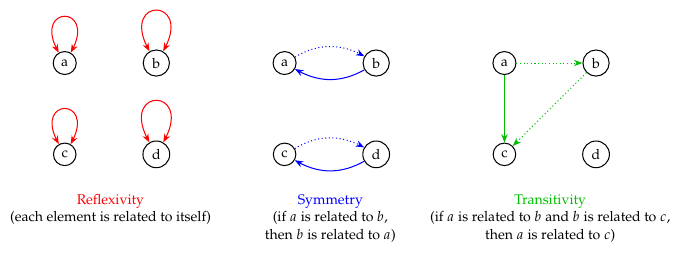
\includegraphics[scale=.4]{lecture-note-1}
		\caption{Set Theory (Equivalence Relation)}
	\end{figure}
	
	\begin{figure}[h!]\centering
	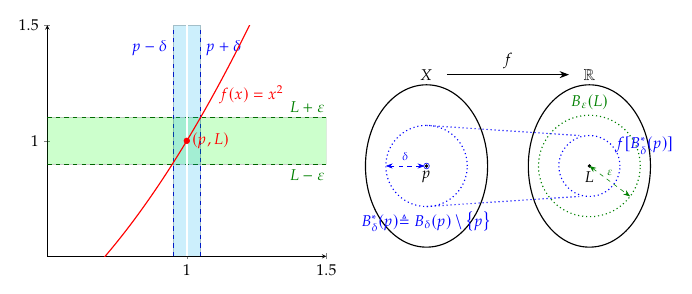
\includegraphics[scale=.4]{lecture-note-4}
	\caption{Advanced Calculus ($\varepsilon-\delta$ method)}
	\end{figure}

	\begin{figure}[h!]\centering
	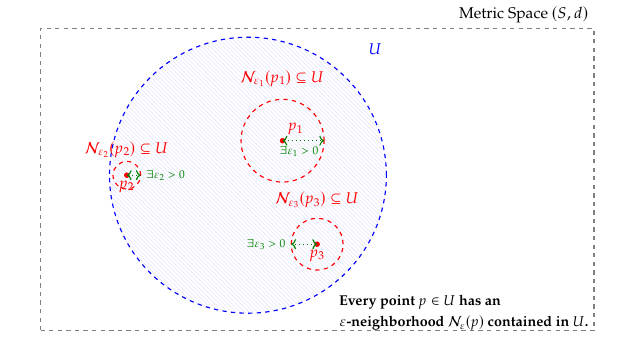
\includegraphics[scale=.4]{lecture-note-3}
	\caption{Topology (Neighborhood)}
	\end{figure}

	\newpage
	%--------- Course Outline ---------
	\section*{Course Outline / 세미나 주요 내용 (일부만 기재)}
\begin{enumerate}
%	[label=\textbf{Week \arabic*:}, leftmargin=*, itemsep=1em]
\item[] \textbf{Set Theory / 집합론} \\
Topics: Basic set operations, functions, relations, and cardinality. \\
주제: 집합의 기본 연산, 함수, 관계, 기수

\item[] \textbf{Advanced Calculus (Analysis) / 고급 미적분학 (해석학)} \\
Topics: Structure of the real number system, sequences, series, limits, and continuity. \\
주제: 실수 체계의 구조, 수열, 급수, 극한, 연속성.

\item[] \textbf{Topology / 위상수학} \\
Topics: Metric spaces, open and closed sets. \\
%bases for a topology, continuity, and compactness. \\
주제: 거리 공간, 열린 집합 및 닫힌 집합.
%, 위상의 기저, 연속성, 콤팩트성.

%\item[] \textbf{Topology II / 위상수학 II} \\
%Topics: Connectedness, path-connectedness, the fundamental group, and introductory algebraic topology. \\
%주제: 연결성, 경로 연결성, 기본군, 기초 대수적 위상수학.

\item[] \textbf{Linear Algebra / 선형대수학} \\
Topics: Vector spaces, linear transformations, matrices, and systems of linear equations. \\
주제: 벡터 공간, 선형 변환, 행렬, 연립 선형 방정식.

%\item[] \textbf{Linear Algebra II / 선형대수학 II} \\
%Topics: Eigenvalues, eigenvectors, diagonalization, and inner product spaces. \\
%주제: 고유값, 고유벡터, 대각화, 내적 공간.

\item[] \textbf{Abstract Algebra / 추상대수학} \\
Topics: Groups, subgroups, cyclic groups, and group homomorphisms. \\
주제: 군, 부분군, 순환군, 군 준동형.

%\item[] \textbf{Abstract Algebra II / 추상대수학 II} \\
%Topics: Rings, ideals, ring homomorphisms, and an introduction to fields and modules. \\
%주제: 환, 아이디얼, 환 준동형, 필드와 가군 소개.

%\item[] \textbf{Integration of Concepts / 개념의 통합} \\
%Topics: Interdisciplinary projects and advanced topics integrating various mathematical disciplines. \\
%주제: 다양한 수학 분야를 통합하는 학제 간 프로젝트 및 심화 주제.

%\item[] \textbf{Final Review and Assessment / 최종 복습 및 평가} \\
%Topics: Comprehensive review, problem-solving sessions, and final examinations. \\
%주제: 종합 복습, 문제 해결 세션, 최종 평가.
\item[] \textbf{etc}.
\end{enumerate}

\vspace{1em}

\section*{Final Remarks / 마지막 안내}
Mathematics is best learned by discussion and practice. Don’t hesitate to ask questions
and collaborate with your peers. Let’s explore the beauty of mathematics together!\\

\noindent 수학은 토론과 연습을 통해 가장 잘 배울 수 있습니다. 질문을 주저하지 말고, 멤버들과
함께 협력하며 수학의 아름다움을 탐구해 봅시다!
	
\end{document}